\section{Historical Baseline and Tycho Analyses}\label{app:analysis}
Sections D.1--D.3 describe the original November 6 baseline with a 100-action cap per game. Section~\ref{app:followup} records selected November 9 Tycho follow-up cases. Section~\ref{app:continued-audit} reports the baseline after continuation used in the main comparison. Keeping these records separate distinguishes the original 23.16\% result from the final 46.20\% baseline score. Neither the original score decomposition nor the Tycho cases isolates a layer's effect in a whole-game experiment. The original D/R exposure labels below also differ from the layer-design categories used in the main study.

\subsection{Score reconstruction and cap analysis}
The scoring script reconstructed the original 100-action baseline score from the 183 pairs of integer action counts and official human baselines in \code{data/level_results.csv}. It assigned zero to uncompleted levels, calculated completed-level efficiencies using Equation~\eqref{eq:level}, applied the level weights and completion cap, and averaged over 25 games. The reconstructed overall score was 23.16434010\%. Every displayed level and game score matched at its printed precision, and 60 completed levels reached the maximum efficiency of 1.15.

To examine the effect of the 100-action cap, I also calculated a counterfactual in which each level took exactly its official human-baseline action count. I defined the cumulative baseline through level $\ell$ as $B_{g\ell}=\sum_{j=1}^{\ell}b_{gj}$. A level counts as completed in this calculation when $B_{g\ell}\leq100$. I set $d^{H}_{g\ell}=1$ in that case and 0 otherwise. Each completed level had efficiency 1, giving the game score
\[
100\sum_\ell \ell d^{H}_{g\ell}/W_g.
\]
The mean across games was 10.73304473\%. This calculation assumed sequential progression, exact baseline action counts, no exploration overhead, and no resets. It described how the cap interacted with scoring. It did not estimate sampled human performance.

Table~\ref{tab:decomposition} separates the effects of aggregation, level weights, and action efficiency on this original result. Pooled completion gave every level equal weight across all games. Equal-game unweighted completion instead divided each game's completed levels by its own level count, then averaged across games. This gave 37.74921\%. Applying the official level-index weights within each game lowered the mean to 23.28225\%. Applying the observed efficiencies and game completion caps gave 23.16434\% RHAE, a further decrease of 0.11791 percentage points. These were arithmetic recalculations of one run.
\begin{table}[htbp]
\centering\small
\begin{tabularx}{\linewidth}{@{}Yrr@{}}\toprule
Score decomposition & Value (\%) & Change (pp)\\\midrule
Pooled completion $100\sum_g\sum_\ell d_{g\ell}/183$ & 36.61202 & ---\\
Equal-game mean of unweighted completion & 37.74921 & $+1.13718$\\
Equal-game mean of weighted completion & 23.28225 & $-14.46696$\\
RHAE after action efficiency and completion cap & 23.16434 & $-0.11791$\\\bottomrule
\end{tabularx}
\caption{The table decomposes the original 100-action baseline score arithmetically. Each change is the current row minus the preceding row, in percentage points (pp). The changes show the effects of aggregation, level weights, and action efficiency after the game completion cap, respectively. All rows recalculate the same run. I removed and reran no component.}\label{tab:decomposition}
\end{table}


\subsection{Original 100-action game list}
Table~\ref{tab:games} lists all 25 games in the original 100-action evaluation, including the game with zero score. D denotes the original development partition, which included every game with recorded prior exposure. The remaining games were assigned to partitions using a fixed seed and hashes of their full game IDs. R combined the reduced-exposure \texttt{h1} and \texttt{h2} groups from that partition. These labels recorded the original exposure classification; they did not guarantee that R games were unseen, and they differed from the main study's eight-game development group.

In this run, each successful action-selection call produced one model-chosen action, while the controller issued resets. The number of action-selection calls was therefore actions minus resets. The saved scorecard file retains the public replay URLs.
\begin{table}[H]
\centering\small
\setlength{\tabcolsep}{4pt}
\begin{tabularx}{\linewidth}{@{}lcrrrrY@{}}\toprule
Versioned game & Group & RHAE (\%) & Levels & Actions & Resets & Scorecard state\\\midrule
\texttt{ar25-0c556536} & D & 16.67 & 3/8 & 100 & 0 & \texttt{NOT\_FINISHED}\\
\texttt{bp35-0a0ad940} & R & 2.22 & 1/9 & 100 & 3 & \texttt{GAME\_OVER}\\
\texttt{cd82-fb555c5d} & D & 14.29 & 2/6 & 100 & 0 & \texttt{NOT\_FINISHED}\\
\texttt{cn04-2fe56bfb} & R & 14.29 & 2/6 & 100 & 0 & \texttt{NOT\_FINISHED}\\
\texttt{dc22-fdcac232} & R & 4.76 & 1/6 & 100 & 0 & \texttt{NOT\_FINISHED}\\
\texttt{ft09-0d8bbf25} & D & 100.00 & 6/6 & 75 & 0 & \texttt{WIN}\\
\texttt{g50t-5849a774} & D & 3.57 & 1/7 & 100 & 0 & \texttt{NOT\_FINISHED}\\
\texttt{ka59-38d34dbb} & D & 3.11 & 1/7 & 100 & 0 & \texttt{NOT\_FINISHED}\\
\texttt{lf52-271a04aa} & D & 1.82 & 1/10 & 100 & 0 & \texttt{NOT\_FINISHED}\\
\texttt{lp85-305b61c3} & R & 77.78 & 7/8 & 100 & 0 & \texttt{NOT\_FINISHED}\\
\texttt{ls20-9607627b} & D & 10.71 & 2/7 & 100 & 0 & \texttt{NOT\_FINISHED}\\
\texttt{m0r0-492f87ba} & R & 14.29 & 2/6 & 100 & 0 & \texttt{NOT\_FINISHED}\\
\texttt{r11l-495a7899} & R & 71.43 & 5/6 & 100 & 0 & \texttt{NOT\_FINISHED}\\
\texttt{re86-8af5384d} & R & 8.33 & 2/8 & 100 & 0 & \texttt{NOT\_FINISHED}\\
\texttt{s5i5-18d95033} & D & 8.33 & 2/8 & 100 & 0 & \texttt{NOT\_FINISHED}\\
\texttt{sb26-7fbdac44} & R & 58.33 & 6/8 & 100 & 0 & \texttt{NOT\_FINISHED}\\
\texttt{sc25-635fd71a} & D & 27.11 & 3/6 & 100 & 0 & \texttt{GAME\_OVER}\\
\texttt{sk48-d8078629} & D & 8.33 & 2/8 & 100 & 0 & \texttt{NOT\_FINISHED}\\
\texttt{sp80-589a99af} & D & 47.62 & 4/6 & 100 & 1 & \texttt{GAME\_OVER}\\
\texttt{su15-1944f8ab} & D & 6.67 & 2/9 & 100 & 2 & \texttt{GAME\_OVER}\\
\texttt{tn36-ef4dde99} & R & 0.00 & 0/7 & 100 & 1 & \texttt{GAME\_OVER}\\
\texttt{tr87-cd924810} & D & 3.73 & 1/6 & 100 & 0 & \texttt{NOT\_FINISHED}\\
\texttt{tu93-0768757b} & R & 33.33 & 5/9 & 100 & 1 & \texttt{GAME\_OVER}\\
\texttt{vc33-5430563c} & D & 35.71 & 4/7 & 100 & 0 & \texttt{NOT\_FINISHED}\\
\texttt{wa30-ee6fef47} & D & 6.67 & 2/9 & 100 & 0 & \texttt{NOT\_FINISHED}\\
\midrule
All games & & 23.16 & 67/183 & 2,475 & 8 & 1 WIN, 6 GAME\_OVER, 18 NOT\_FINISHED\\\bottomrule
\end{tabularx}
\caption{The table lists all 25 games in the original November 6 baseline, with a 100-action cap per game. It shows scores at scorecard display precision. The final row gives the equal-game mean. Levels are completed levels divided by available levels. D denotes the original development partition. R denotes reduced exposure. Actions include resets. For \texttt{bp35}, \texttt{sp80}, \texttt{su15}, \texttt{tn36}, and \texttt{tu93}, the scorecard showed \texttt{GAME\_OVER}, although the controller reset and continued to the action cap. Only \texttt{sc25} ended in game-over.}\label{tab:games}
\end{table}



\subsection{Platform interaction-tag summaries}
ARC also reported scores by interaction tag. Table~\ref{tab:tags} preserves those platform summaries for the original 100-action baseline. Their aggregation differed from the equal-game RHAE used in the paper.
\begin{table}[H]
\centering\small
\begin{tabular}{@{}lrrrr@{}}\toprule
Platform tag & Tag score (\%) & Levels completed & Actions & Games\\\midrule
\texttt{click} & 24.10 & 21 & 700 & 7\\
\texttt{keyboard} & 6.56 & 6 & 400 & 4\\
\texttt{keyboard\_click} & 19.59 & 34 & 1,300 & 13\\\bottomrule
\end{tabular}
\caption{The table preserves the platform's interaction-tag summaries for the original 100-action baseline. ARC's tag scores are not means of the corresponding game scores, so they are not directly comparable with the equal-game 23.16434\% RHAE. The tag grouping covers 24 games and omits \texttt{ft09}. The full evaluation included all 25.}\label{tab:tags}
\end{table}


\subsection{Follow-up provenance and reference context}\label{app:followup}
I archived the selected Tycho follow-up cases in \code{reports/tycho_opus55_matched_v1} at commit \code{5fd62ecc727963e89c78bf036b97bd03184e4b1f}. The human-readable report was \code{reports/tycho_opus55_matched_v1_results.md}. In the paper source, \code{data/tycho/results.json} preserved the structured outcomes. The files \code{matched_trace.json} and \code{final_trace.json} preserved the action sequences and expected frame hashes. Their replay manifests recorded closed competition-mode cards with no replay failure. These API replays checked deterministic action sequences. They were not new inference trials.

The original 100-action baseline scorecard was \href{https://arcprize.org/scorecards/09cc9d25-ec26-4f26-98f8-9cbd60ec69d7}{\texttt{09cc9d25}} \citep{scorecard2026reported}. The two-game Tycho replay card was \href{https://arcprize.org/scorecards/ac6e3999-e5e4-4488-b981-9d6d80eff73f}{\texttt{ac6e3999}} \citep{scorecard2026tychocard}. For the Tycho \texttt{bp35} continuation, the 427-action checkpoint replay was \href{https://arcprize.org/replay/a8d9ab0a-653c-4e47-8f29-d932551cdd4d}{\texttt{a8d9ab0a}} \citep{scorecard2026bp35checkpoint}, and the completed 474-action replay was \href{https://arcprize.org/replay/b642c1f4-99b6-491f-8e84-813ca4634314}{\texttt{b642c1f4}} \citep{scorecard2026bp35win}. The completed replay's 100\% game score applied to \texttt{bp35} alone.

The three run specifications shared the policy source SHA-256 hash \code{267b1c28f129d4492f1c82a9f503cf3eb5b47c9c836d55e8c8adb3c109eef242}. The recorded overrides first changed \code{TYCHO_MAX_GAME_ACTIONS} from 100 to 0. Here, zero removed the whole-game action cap while retaining the per-level limit of five times the human-baseline action count. They then changed \code{TYCHO_MAX_INFERENCE_COST_PER_GAME} from 100 to 115 US dollars, raising the cumulative inference-cost limit for the game.

The continuation's final manifest reported cumulative usage of 19,450,893 uncached-input, 44,953,313 cache-read, 1,938,558 cache-write, and 558,762 output tokens. Under the archived price schedule,
\[
K=(4N_{\mathrm{uncached}}+0.20N_{\mathrm{read}}+5N_{\mathrm{write}}+20N_{\mathrm{out}})/10^6,
\]
these counts gave a usage cost of \$107.6622646 at the archived API prices. Promotional credits paid for the API usage. Here $K$ is in US dollars. Throughput and builder-activity fields in a resumed manifest could cover only the resumed segment. Accounting for earlier activity therefore required the cumulative result and the complete action record.

For context, ARC Prize published GPT-6 Astra Public Demo sessions using its Provider Adapter harness \citep{arc2026astra}. The archived high-effort \texttt{bp35} session used 488 actions, with per-level counts of 15, 40, 34, 23, 31, 103, 57, 71, and 114 across the nine levels. Across six published effort settings, totals ranged from 430 to 516 actions. Table~\ref{tab:bp35-levels} places the high-effort session beside the Tycho result and official human baselines.

The Astra and Tycho runs differed in model, harness, backend, inference resources, and exposure conditions. Their action counts provided a reference scale. They did not establish superiority or cost efficiency. The archived external session summary, \code{data/tycho/astra_reference.json}, was separate from my experiments.

\begin{table}[H]
\centering\small
\begin{tabular}{@{}lrrrrrrrrrr@{}}\toprule
Level & 1 & 2 & 3 & 4 & 5 & 6 & 7 & 8 & 9 & Total\\\midrule
Official human baseline & 21 & 48 & 44 & 38 & 33 & 87 & 86 & 131 & 163 & 651\\
Tycho + Opus 5.5 & 15 & 49 & 34 & 23 & 35 & 68 & 54 & 57 & 139 & 474\\
Astra, adapter, high & 15 & 40 & 34 & 23 & 31 & 103 & 57 & 71 & 114 & 488\\\bottomrule
\end{tabular}
\caption{The table gives scorer-counted actions by level for \texttt{bp35}. The agent totals include resets. The Astra row is an external reference under different conditions, not a matched model comparison.}\label{tab:bp35-levels}
\end{table}

Running \texttt{python3 verify\_followup.py} reconstructed the follow-up scores and costs, compared the 100-action prefix, checked replay summaries, and checked that the two run-specification changes affected only the recorded budgets. The script made no model or network call. The compressed inference records, model-generated analyses, and the executable world-model artifact remained in the GitHub archive at the cited commit. The model-generated notes and feature attributions were not validated rules or causal evidence.



\subsection{Baseline after continuation and final replay}\label{app:continued-audit}
The baseline used in the main comparison extended the original runs under the archived per-game caps. It completed 125 of 183 levels, won seven games, and used 16,560 actions, including 127 resets. Its third competition-mode replay, card \code{0f882c2e-0451-41bd-86c5-211a54785c56}, confirmed 46.19821647\% RHAE and matched all 16,560 recorded observations \citep{dai2026baselinefinalcard}. Earlier cards recorded intermediate checkpoints. Table~\ref{tab:continued-games} gives the final per-game results.

\begin{table}[H]
\centering\small
\setlength{\tabcolsep}{4pt}
\begin{tabular*}{\linewidth}{@{\extracolsep{\fill}}lrrrrr@{}}\toprule
Versioned game & \shortstack{Replay-confirmed\\RHAE (\%)} & Levels & Actions & Cap & Resets\\\midrule
\texttt{ar25-0c556536} & 100.00 & 8/8 & 393 & 750 & 0\\
\texttt{bp35-0a0ad940} & 3.63 & 4/9 & 700 & 700 & 22\\
\texttt{cd82-fb555c5d} & 14.29 & 2/6 & 200 & 200 & 1\\
\texttt{cn04-2fe56bfb} & 47.62 & 4/6 & 800 & 800 & 4\\
\texttt{dc22-fdcac232} & 40.34 & 4/6 & 1,250 & 1,250 & 4\\
\texttt{ft09-0d8bbf25} & 100.00 & 6/6 & 75 & 100 & 0\\
\texttt{g50t-5849a774} & 10.71 & 2/7 & 900 & 900 & 6\\
\texttt{ka59-38d34dbb} & 10.16 & 3/7 & 750 & 750 & 4\\
\texttt{lf52-271a04aa} & 8.54 & 4/10 & 1,350 & 1,350 & 3\\
\texttt{lp85-305b61c3} & 100.00 & 8/8 & 124 & 400 & 0\\
\texttt{ls20-9607627b} & 10.71 & 2/7 & 800 & 800 & 6\\
\texttt{m0r0-492f87ba} & 14.29 & 2/6 & 1,150 & 1,150 & 7\\
\texttt{r11l-495a7899} & 92.35 & 6/6 & 159 & 250 & 1\\
\texttt{re86-8af5384d} & 58.33 & 6/8 & 1,300 & 1,300 & 3\\
\texttt{s5i5-18d95033} & 85.34 & 8/8 & 486 & 650 & 0\\
\texttt{sb26-7fbdac44} & 100.00 & 8/8 & 127 & 150 & 0\\
\texttt{sc25-635fd71a} & 27.11 & 3/6 & 350 & 350 & 6\\
\texttt{sk48-d8078629} & 15.93 & 4/8 & 1,100 & 1,100 & 3\\
\texttt{sp80-589a99af} & 47.62 & 4/6 & 550 & 550 & 11\\
\texttt{su15-1944f8ab} & 45.89 & 7/9 & 400 & 400 & 7\\
\texttt{tn36-ef4dde99} & 19.11 & 4/7 & 350 & 350 & 2\\
\texttt{tr87-cd924810} & 27.09 & 4/6 & 450 & 450 & 1\\
\texttt{tu93-0768757b} & 62.20 & 8/9 & 500 & 500 & 24\\
\texttt{vc33-5430563c} & 72.27 & 7/7 & 446 & 450 & 2\\
\texttt{wa30-ee6fef47} & 41.44 & 7/9 & 1,850 & 1,850 & 10\\
\midrule
All games & 46.20 & 125/183 & 16,560 & 17,500 & 127\\\bottomrule
\end{tabular*}
\caption{The table gives the final baseline results under the archived per-game action caps, which competition-mode replay confirmed. Levels are completed levels divided by available levels. Actions include resets. The All games row totals the counts and caps and gives the equal-game RHAE of 46.20\%. The baseline won seven games.}\label{tab:continued-games}
\end{table}

For the final baseline \texttt{wa30} run, per-level action counts were $(36,59,187,462,110,70,244,682,0)$, with seven levels completed. The eighth entry counts actions used on the unfinished eighth level; the final zero indicates that level nine was never reached. The corresponding human-baseline counts were $(71,119,183,98,368,68,79,442,415)$. The game score was 41.44187593\%.

Across all games, the baseline after continuation had a mean weighted completion cap of 54.28600289\%. This was the mean of the highest scores permitted by the levels completed in each game, before losses from action inefficiency. Later levels received greater weight, and each game contributed equally to this mean, so it differed from the unweighted completion fraction of 125/183. Its RHAE was 8.08778642 percentage points below that cap after accounting for action efficiency. These calculations described the extended baseline. They did not isolate a policy change.

The original \code{verify_continuation.py} retained its historical checkpoint transcription and offline extension arithmetic. For the final comparison, \code{verify_layered.py} read the final baseline and layered replay records and checked the full 25-game results and reported usage. These arithmetic checks did not launch model runs or independently verify the private restoration logs.


\section{Step Counters and the No-Effect Examples}\label{app:no-effect-traces}
Figure~\ref{fig:step-counter} shows step counters in three games and the cells the harness ignored when it compared boards. Figure~\ref{fig:no-effect-examples} shows two examples from the evaluated runs. Because the harness ignored step-counter cells when comparing final boards, it classified both actions as no-effect actions. The records below give the frame counts and the lessons written by the model.

\begin{figure}[htbp]
\centering
\begin{tabular}{@{}c@{\hspace{8pt}}c@{\hspace{8pt}}c@{}}
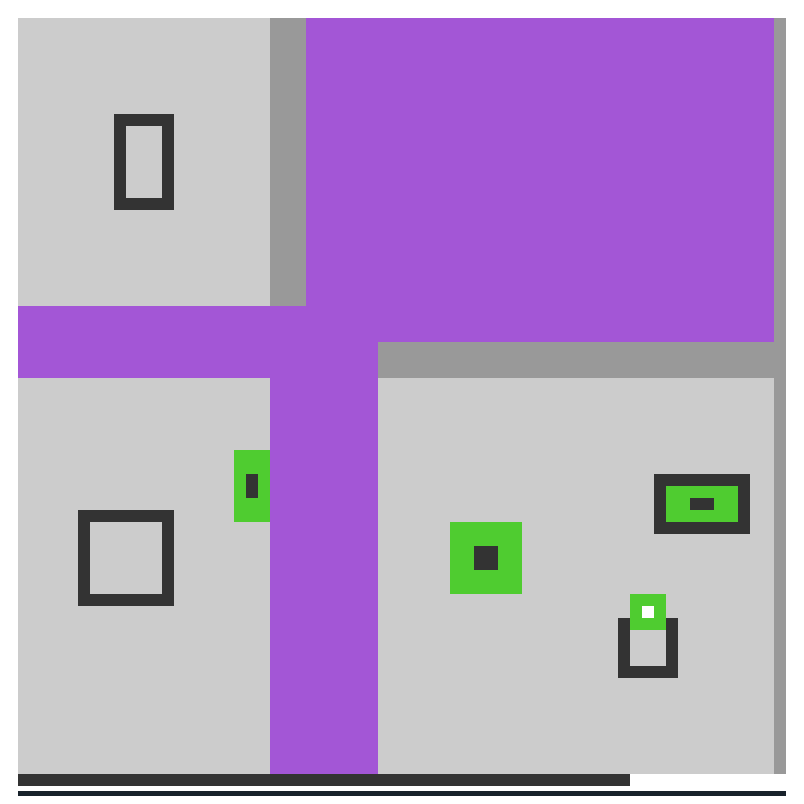
\includegraphics[width=0.29\linewidth]{figures/runs/step-counter-a.png} &
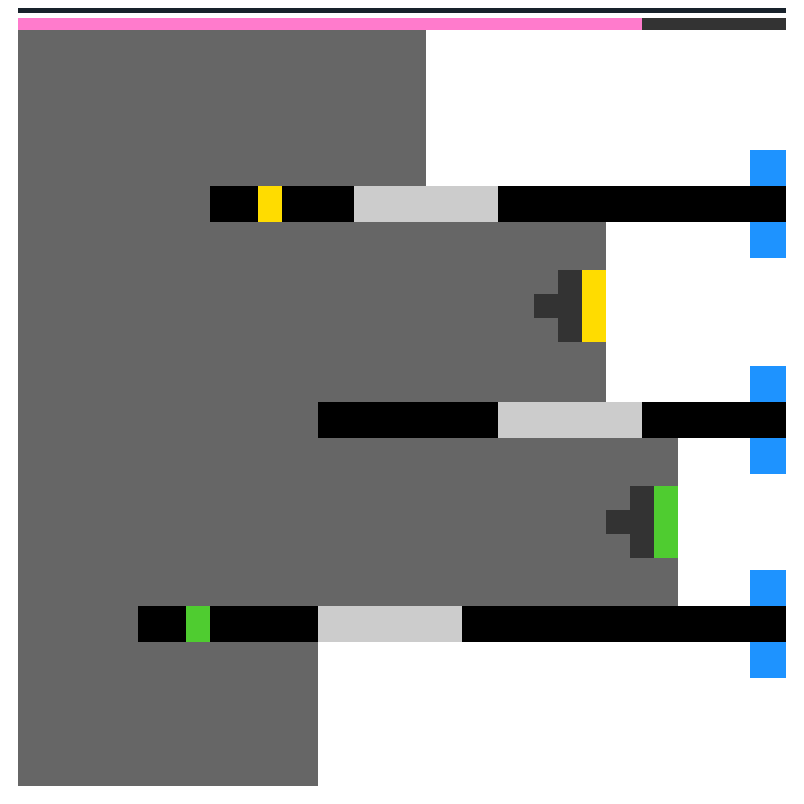
\includegraphics[width=0.29\linewidth]{figures/runs/step-counter-b.png} &
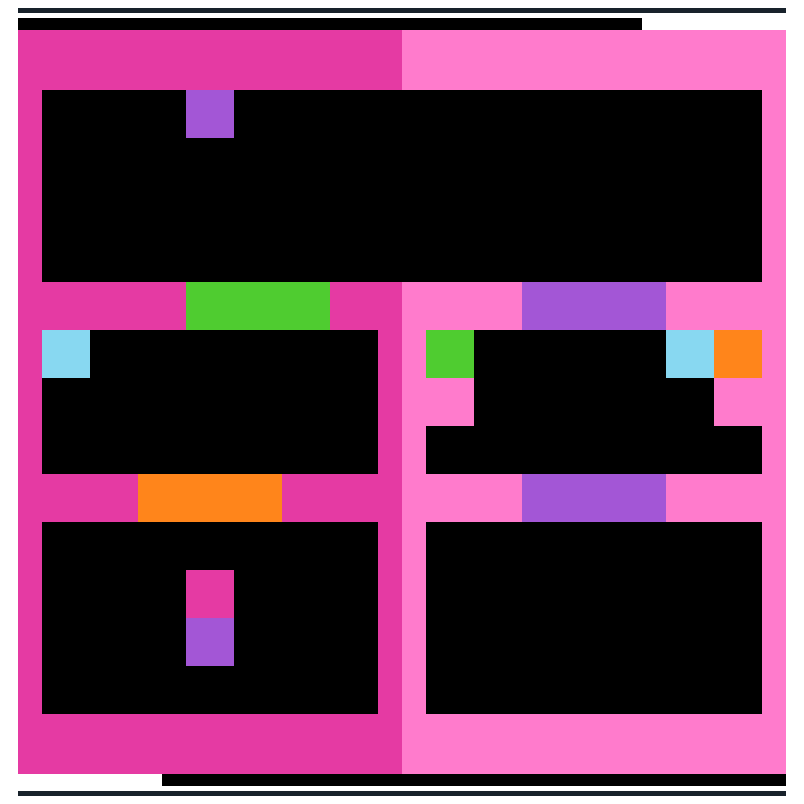
\includegraphics[width=0.29\linewidth]{figures/runs/step-counter-c.png}\\[1pt]
\footnotesize (a) \texttt{ka59}, level 2: bottom row & \footnotesize (b) \texttt{vc33}, level 5: top row & \footnotesize (c) \texttt{m0r0}, level 5: top and bottom rows
\end{tabular}\\[7pt]
\begin{tabular}{@{}r@{\hspace{8pt}}c@{}}
\footnotesize After action 30 & \raisebox{-0.3\height}{\board[0.74\linewidth]{step-counter-d.png}}\\[5pt]
\footnotesize After action 53 & \raisebox{-0.3\height}{\board[0.74\linewidth]{step-counter-e.png}}\\[5pt]
\footnotesize After action 77 & \raisebox{-0.3\height}{\board[0.74\linewidth]{step-counter-f.png}}
\end{tabular}\\[3pt]
{\footnotesize (d) Close-up of the bottom four rows in (a) at three points during level 2}
\caption{\textbf{Some games show a bar that changes as the agent takes actions.} These examples come from the evaluated layered runs. The bar is on the bottom row in (a), the top row in (b), and both the top and bottom rows in (c). The dark lines drawn outside the boards mark the cells the harness ignored when comparing boards. The figure adds these lines. Panel (d) shows a close-up of the bar in (a). Its dark section shrank from 63 cells after action 30 to 51 after action 53 and 39 after action 77. The harness can miss a counter, and some games have no visible counter \citep{dai2026runfigures}.}\label{fig:step-counter}
\end{figure}


\begin{figure}[htbp]
\centering
\begin{tabular}{@{}c@{\hspace{8pt}}c@{}}
\board[0.235\linewidth]{lessons-no-effect-a.png} & \board[0.235\linewidth]{lessons-no-effect-b.png}\\[1pt]
\footnotesize Before action 11, click ringed & \footnotesize After it
\end{tabular}\\[2pt]
{\small (a) \texttt{ka59}, level 1. A click with no final change outside the step counter}\\[8pt]
\begin{tabular}{@{}c@{\hspace{8pt}}c@{\hspace{8pt}}c@{\hspace{8pt}}c@{}}
\board[0.235\linewidth]{frames-between-a.png} & \board[0.235\linewidth]{frames-between-b.png} &
\board[0.235\linewidth]{frames-between-c.png} & \board[0.235\linewidth]{frames-between-d.png}\\[1pt]
\footnotesize Before action 343, click ringed & \footnotesize Frame 5 of 15 & \footnotesize Frame 10 of 15 & \footnotesize Last frame
\end{tabular}\\[2pt]
{\small (b) \texttt{dc22}, level 5. The board changed and changed back}
\caption{\textbf{An action can change the board and then return it to its earlier appearance.} (a) In \texttt{ka59}, level 1, the boards before and after the click differed only in the step counter. (b) In \texttt{dc22}, level 5, the animation changed the board before the final frame returned to its earlier appearance, apart from the counter. The harness classified both actions as no-effect actions because it ignored counter cells in this comparison. Sections~\ref{app:ka59-click} and~\ref{app:dc22-animation} give the frame counts and the model's lessons \citep{dai2026runfigures}.}\label{fig:no-effect-examples}
\end{figure}


\subsection{A click in \texttt{ka59}, level 1}\label{app:ka59-click}
The click at action 11 changed only one bottom-row step-counter cell. After one additional action, the model wrote, ``ACTION6 only does something when it clicks a cell of a 3x3 e-box, which it then selects.''

\subsection{An animation in \texttt{dc22}, level 5}\label{app:dc22-animation}
The click at action 343 returned 15 animation frames. Relative to the board before the click, 38 cells differed in frame 5, 1,575 in frame 10, and 2,830 in frame 14. The final frame differed only in two step-counter cells.

The model received the final board and a summary of the intermediate frame with the most changed cells. From this evidence, it wrote, ``A control that toggles same-colour bridges between solid and checkered will not run while the e marker stands on a bridge that would become checkered. The toggle plays out in the intermediate frames and then reverts, so the final board is unchanged.'' This was the model's interpretation, not a verified game rule. The letter e is a color code \citep{dai2026runfigures}.

\FloatBarrier
\section{Continuation Checks and Call Accounting}\label{app:continuation}
If an interruption stopped a run, the runner used its saved model replies and game observations to restore its progress. Before requesting a new decision, it reconstructed the input shown to the model at each earlier decision and checked that it matched the saved input exactly. It also checked the recorded actions, observations, model name, settings, and action caps. The public experiment plans included a unique identifier, or hash, for each code file to record the exact version used. The resumed run continued from its earlier progress, and its previous actions still counted toward the same cap. It was therefore part of the original trial. I stored the complete logs of model inputs and replies locally and did not include them in the public archive.

Across the 25 layered runs, the harness rejected 461 of 11,111 replies (4.1\%). Each rejected reply tried to add a rule to the full 12-rule list without identifying an existing rule to replace. Five additional replies had the same error, but the model returned them during decisions that an interruption prevented from finishing. When the run continued, the runner started the interrupted decision again. The reported reply and token totals excluded those five replies.

Separately, 97 calls exceeded the time limit without returning a reply. A retry followed 77 of them. The other 20 exhausted the retry allowance and stopped execution. I later resumed some runs from their saved records, so a single run could account for more than one of these stops. Eight other calls failed because a subscription reached its usage limit, and two failed because there was no connection. I counted these events in the local logs using the public script \code{research/level_brief_v1/whole_verify.py} and archived the counts \citep{dai2026logcounts,dai2026wholeverify}.
